\newcommand{\SystemFigure}{%
\begin{figure*}[t]
\centering
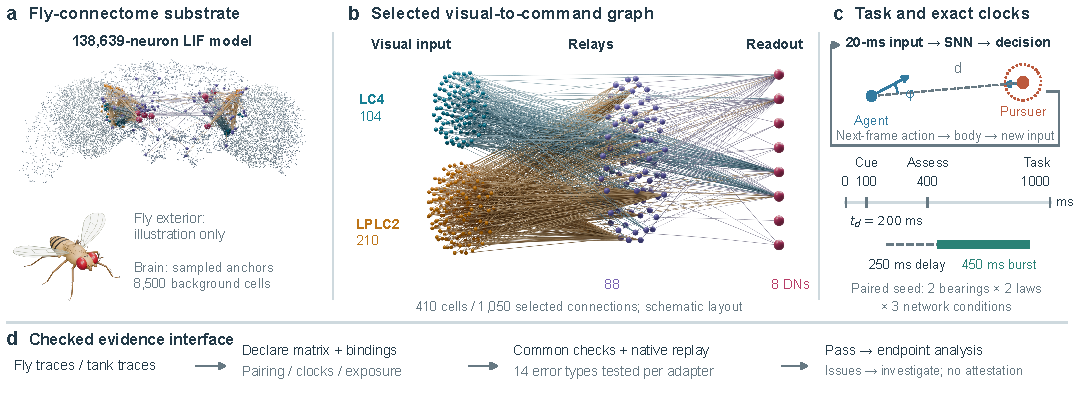
\includegraphics[width=\textwidth]{figs/evidence_v10_overview.pdf}
\caption{System and checked assessment interface. (a,b) Representative model anchors, an illustrative fly and a selected 410-cell/1,050-connection graph. The layout is schematic, not measured neurites or the complete recurrent graph. (c) Sampled feedback and exact burst events; $t_d=200$\,ms is illustrative. (d) Native traces enter common checks and independent replay before endpoint analysis.}
\label{fig:v10f-system}
\end{figure*}}
\newcommand{\ReuseCaption}{Cross-plant reuse and predefined error challenges. (a) First registered tank seed, high inflow, proportional law; level axis is zoomed, safe interval $[0.2,0.8]$. All 96 example tasks remain safe. (b) A requested outflow first changes at 0.60\,s and applies at 0.75\,s, between 100-ms frame boundaries. (c) Eleven common-checker and three native-only cases are detected per adapter, not a general coverage estimate.}
\newcommand{\WarningCaption}{Frozen secondary warning operating points. Rows state contact/success denominators; RF-0/A/B contain 24/12/12 independent seed clusters. Markers show missed-contact and false-alarm rates with pointwise 95\% whole-seed bootstrap CIs. Activity is two-sided; the forecast holds the current command using exact simulated state. Zero observed misses and class-conditional intervals do not establish zero population risk.}
\iffourfigures
\newcommand{\reuseRef}{Fig.~\ref{fig:v10f-reuse}}
\newcommand{\warningRef}{Fig.~\ref{fig:v10f-warning}}
\newcommand{\ReuseFigure}{%
\begin{figure}[t]\centering
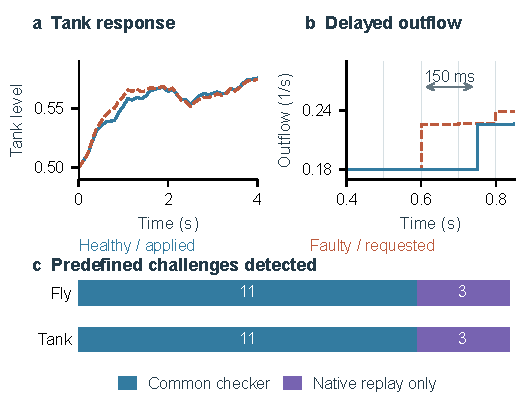
\includegraphics[width=\columnwidth]{figs/v10f_reuse.pdf}
\caption{\ReuseCaption}\label{fig:v10f-reuse}
\end{figure}}
\newcommand{\WarningFigure}{%
\begin{figure}[t]\centering
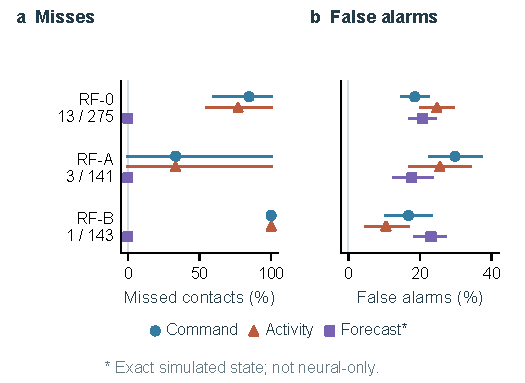
\includegraphics[width=\columnwidth]{figs/v10f_warning.pdf}
\caption{\WarningCaption}\label{fig:v10f-warning}
\end{figure}}
\else
\newcommand{\reuseRef}{Fig.~\ref{fig:v10f-reuse} (left)}
\newcommand{\warningRef}{Fig.~\ref{fig:v10f-warning} (right)}
\newcommand{\ReuseFigure}{%
\begin{figure*}[t]\centering
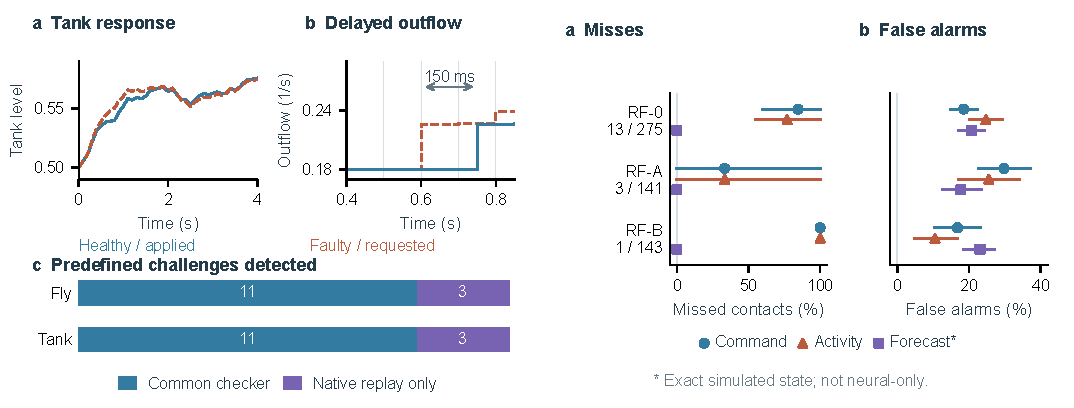
\includegraphics[width=\textwidth]{figs/v10f_reuse_warning.pdf}
\caption{\emph{Left:} \ReuseCaption\ \emph{Right:} \WarningCaption}
\label{fig:v10f-reuse}\label{fig:v10f-warning}
\end{figure*}}
\newcommand{\WarningFigure}{}
\fi
\newcommand{\TransferFigure}{%
\begin{figure*}[t]\centering
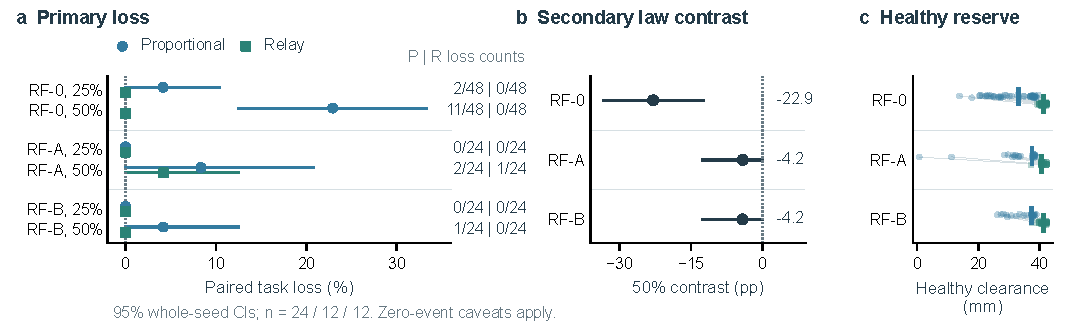
\includegraphics[width=\textwidth]{figs/v10f_rf.pdf}
\caption{Independent RF campaigns. (a) Primary healthy-to-fault losses and P/R loss counts; all healthy tasks succeed and no gains occur. (b) Prespecified secondary relay-minus-proportional net-loss contrast at 50\% deletion, in percentage points. Pointwise 95\% CIs resample whole seeds within each map ($n=24/12/12$), conditional on saved calibrations. (c) All paired healthy minimum-clearance observations, with median bars, show unequal reserve. Maps share a prior but differ in draws, recalibration and test cohorts; differences are not an isolated RF effect.}
\label{fig:v10f-transfer}
\end{figure*}}
